\documentclass{beamer}

\usetheme{Dresden}

\usepackage[english]{babel}
\usepackage[T1]{fontenc}

\title{Assignment 4 -  3}

\subtitle{Algorithms for Geographic Data}

\author[Group 10]{
	Tim van Dalen (0744839)
	\and
	Bram Kohl (0746107)
	\and
	Bart van Wezel (0740608)
}

\institute[TU/e] % (optional, but mostly needed)
{
    WIS\\
	Eindhoven University of Technology
}

\date{\today}


\subject{Algorithms for Geographic Data}


\catcode`\^^I=13
\catcode`\^^M=13

\newcounter{linenumber}

\newenvironment{sourcecode}{\begingroup%
\setcounter{linenumber}{0}%
\def\algorithm##1{\setcounter{linenumber}{0}\medskip \textbf{Algorithm} \textsc{##1} \parskip=0pt\everypar={\parskip=0pt\stepcounter{linenumber}\rlap{\scriptsize{\thelinenumber}}\qquad}}%
\def\event##1{\setcounter{linenumber}{0}\medskip \textbf{##1:} \parskip=0pt\everypar={\parskip=0pt\stepcounter{linenumber}\rlap{\scriptsize{\thelinenumber}}\qquad}}%
%
\def\comment##1{\textit{//##1}}%
\def\qif##1{\textbf{if} ##1}%
\def\qifdefined##1{\textbf{if} ##1 \textbf{defined}}%
\def\qifndefined##1{\textbf{if} ##1 \textbf{not defined}}%
\def\qelse{\textbf{else}}%
\def\qelseif##1{\textbf{else if ##1}}%
\def\for##1{\textbf{for} ##1}%
\def\foreach##1{\textbf{for each} ##1}%
\def\qdo{\textbf{do}}%
\def\while##1{\textbf{while} ##1}%
\def\return##1{\textbf{return} ##1}%
\def\break{\textbf{break}}%
\def\qglobal##1{\textbf{global} ##1}%
\def\qsend##1{\textbf{send} \emph{##1}}%
\def\qreceive##1{\textbf{receive} \emph{##1}}%
\def\qbegin{\textbf{begin}}
\def\qend{\everypar={}\textbf{end}}
\def\runningtime##1{\hfill ##1}
\catcode`\^^I=13%
\catcode`\^^M=13%
\def^^I{\qquad}%
\def^^M{\par}%
}{\endgroup}

\catcode`\^^I=10
\catcode`\^^M=5


\beamertemplatenavigationsymbolsempty
\begin{document}

	\begin{frame}
		\titlepage
	\end{frame}
	
	\begin{frame}
		\centering
		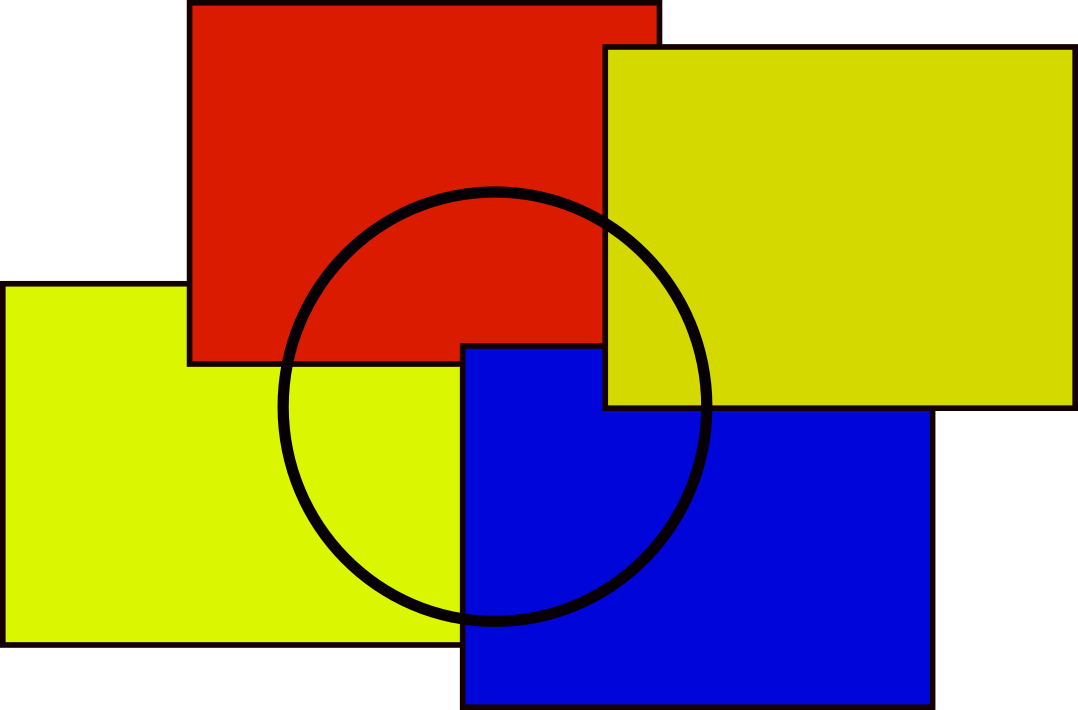
\includegraphics[width=\textwidth]{necklace1}
	\end{frame}
	\begin{frame}
		\centering
		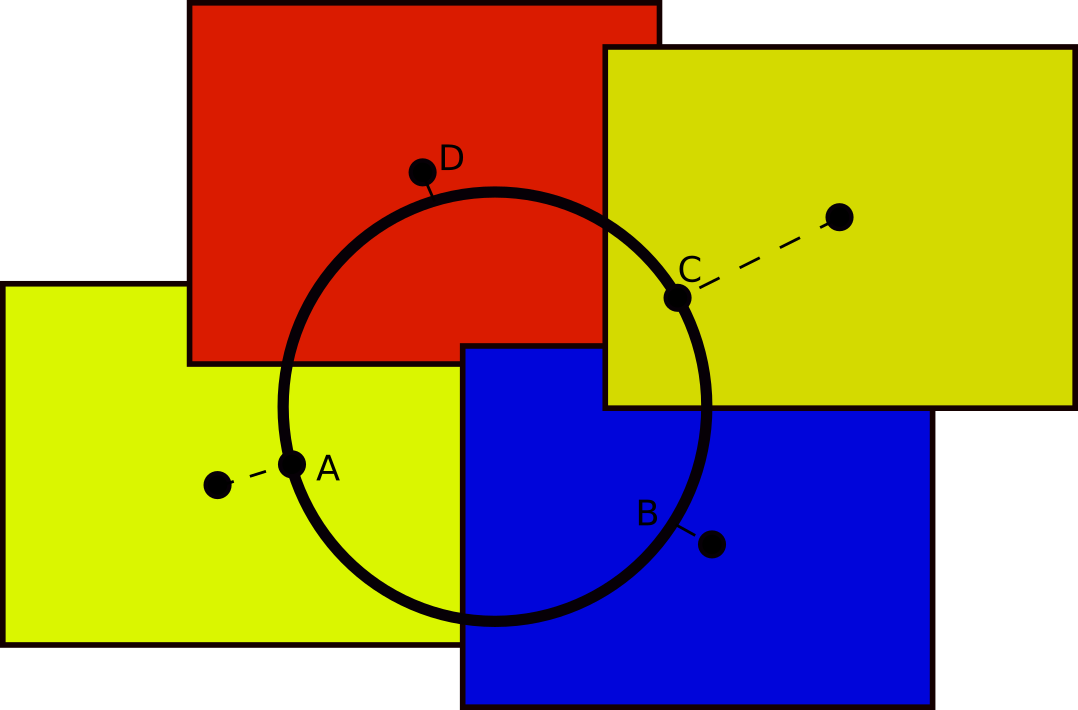
\includegraphics[width=\textwidth]{necklace2}
	\end{frame}
	\begin{frame}
		\centering
		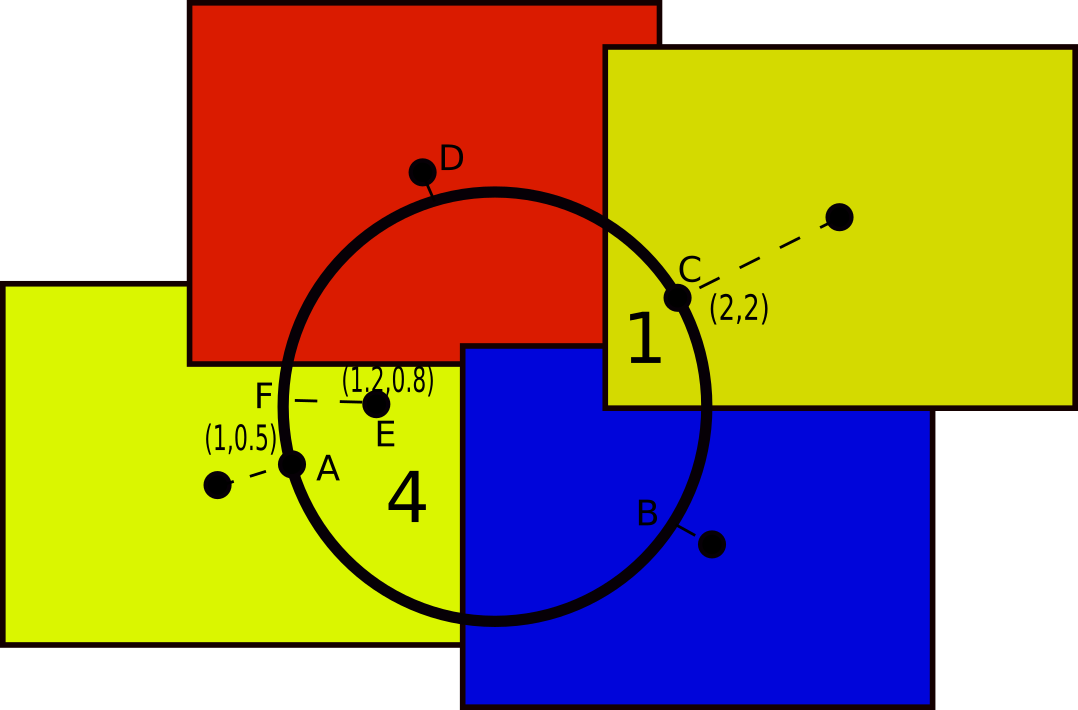
\includegraphics[width=\textwidth]{necklace3}
	\end{frame}
	
	
	\begin{frame}
		\begin{itemize}
			\item Spatially informative
			\item Continuous
		\end{itemize}
	\end{frame}
	
	
\end{document}
